\begin{ZhChapter}

\chapter{Introduction}

After several decades of development, deep learning \cite{deepLearning} technology has achieved significant breakthroughs in the last ten years, largely due to the remarkable improvements in GPU computational power. Consequently, the predictive and analytical capabilities of models have achieved substantial advancements. Numerous models have been launched by major companies and applied in practical scenarios, leading to significant changes in our daily lives.

The model training process can be broadly divided into several key steps: collecting data and organizing it into datasets, partitioning the datasets into training and validation sets as needed, initializing model parameters, evaluating the performance of the model, adjusting the model parameters, and repeating the training until the target is achieved or computational resources are exhausted. During the evaluation of the model's performance, we use a function called the loss function\cite{janocha2017lossfunctionsdeepneural}. Its purpose is to calculate the difference between the model's predicted results and the ground truth, which helps model adjust its parameter to better fit the target. Therefore, different loss functions can influence the direction of model adjustments, significantly impacting the final outcomes of the model.

However, the design of a loss function is often closely related to the propose of the model\cite{lossFunctionMakeDifference}. In other words, different models may require experts from specific fields to assist in designing the loss function to enhance the speed and effectiveness of model training. Nevertheless, recent research has shown that it's feasible to use genetic algorithm (GA) \cite{geneticProgramming} to automatically generate loss functions. Due to the domain-independent nature of GA, it allows us to develop an algorithm that can automatically create the required loss function without needing specialized knowledge in that particular field. However, this method typically requires a significant amount of time and computational resources.

Given the rapid flow of information in today's society, we often need a quick way to find the necessary loss function to optimize the training process of the model. This paper proposes an efficiency-oriented GA, aiming to reduce the time required for GA to search for the optimal algorithm while maintaining the same level of effectiveness.

The structure of this paper is as follows: Chapter 2 is related work. This chapter provides a detailed illustration to the development and history of GA, the detailed description of the loss function and how they collaborate with deep learning model, and how loss functions are randomly generated via GA. Chapter 3 is proposed algorithm and main methodology. In this chapter, we will explain the architecture of the algorithm implemented in this paper. After that, we will then describe the experimental environment setup and the initial parameter values. Finally, we will present the methods and procedures used in this paper. Chapter 4 is results analysis. This section will show the detail parameter settings among all compared peer-algorithm. After that, we will present the analysis of the results by organizing the experimental results into charts and figures. Finally, we will explain the outcomes and analyze why our algorithm can achieve the similar result while decreasing the usage of computational resources. Chapter 5 is conclusion and future work. In this chapter, we will provide the conclusion of this paper by outlining the contribution we have made so far. After that, we would like to discuss potential directions for future research or possible way to apply this algorithm in practical.
% \section{研究動機與背景(小標)}

% \begin{equation} 
%     \mbox{$x = \dfrac{-b\pm\sqrt{b^2-4ac}}{2a}$}
% \end{equation}

% \subsection{研究背景(小小標)}

% \text 背景內文背景內文背景內文背景內文,背景內文背景內文背景內文背景內文背景內文背景內文,如表 1.1 所示。

% \begin{table*}[htbp]
%     \centering
%     \caption{表格範例標題} \label{tab: complexity}
%     \makebox[\linewidth][c]{
%     \renewcommand\arraystretch{1.2}{
%         \begin{tabular}{| l | c  c  c  c |}
%         \hline
%         Protocol & $P$ & $CS_1$ & $CS_2$ & $RG$ \\
%         \hline
%         SD & $O(1)$, $O(1)$, N/A & $O(n-t)$, $O(1)$, N/A & $O(n-t)$, $O(1)$, N/A & $O(1)$, $O(n)$, $O(n)$ \\
%         MSSMul & $O(1)$, $O(1)$, N/A & $O(n-t)$, $O(n)$, $O(1)$ & $O(n-t)$, $O(n)$, N/A & $O(1)$, $O(n)$, $O(n)$ \\
%         MSSAdd & $O(1)$, $O(1)$, N/A & $O(n-t)$, $O(n)$, $O(1)$ & N/A, N/A, N/A & $O(1)$, $O(n)$, $O(n)$ \\
%         SC & $O(1)$, $O(1)$, N/A & $O(n-t)$, $O(n)$, $O(1)$ & $O(n-t)$, $O(n)$, N/A & $O(1)$, $O(n)$, $O(n)$ \\
%         \hline 
%         \end {tabular}
%     }}
% \end {table*}

% \subsubsection{研究動機(小小標)}

% \begin{equation} 
%     \mbox{$(1+x)^n = 1 + \dfrac{nx}{1!} + \dfrac{n(n-1)x^2}{2!}$}
% \end{equation}

% 動機動機動機動機,動機動機動機動機動機動機動機動機動機動機動機動機,動機動機動機動機動機動機動機動機。

% 動機動機動機動機動機動機動機動機,動機動機動機動機動機動機動機動機動機動機動機動機。動機動機動機動機動機動機動機動機,動機動機動機動機動機動機動機動機動機動機動機動機。動機動機動機動機動機動機動機動機,動機動機動機動機動機動機動機動機動機動機動機動機,如圖 1.1、圖 1.2 所示。

% \begin{figure*}[htbp]
%     \centering
%     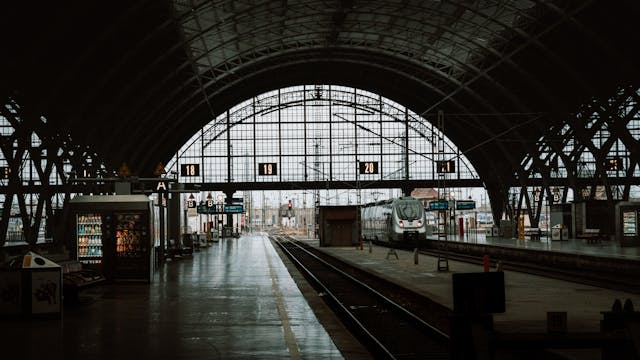
\includegraphics[width = 1\textwidth]{image.jpeg}
%     \caption{Cool train station}
%     \label{fig: image}
% \end{figure*}

% \begin{figure*}[htbp]
%     \centering
%     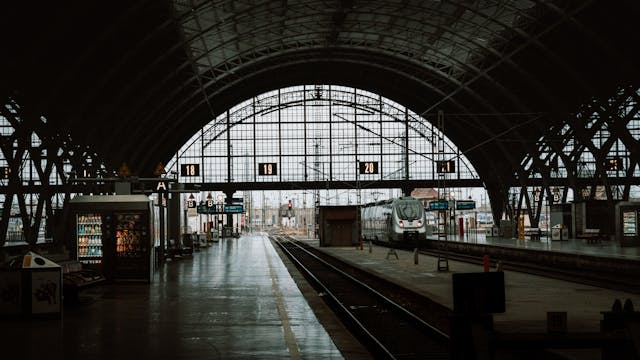
\includegraphics[width = 1\textwidth]{image.jpeg}
%     \caption{Cool train station}
%     \label{fig: image}
% \end{figure*}

% \begin{table*}[htbp]
%     \centering
%     \caption{表格範例標題} \label{tab: complexity}
%     \makebox[\linewidth][c]{
%     \renewcommand\arraystretch{1.2}{
%         \begin{tabular}{| l | c  c  c  c |}
%         \hline
%         Protocol & $P$ & $CS_1$ & $CS_2$ & $RG$ \\
%         \hline
%         MSSMul & $O(1)$, $O(1)$, N/A & $O(n-t)$, $O(n)$, $O(1)$ & $O(n-t)$, $O(n)$, N/A & $O(1)$, $O(n)$, $O(n)$ \\
%         MSSAdd & $O(1)$, $O(1)$, N/A & $O(n-t)$, $O(n)$, $O(1)$ & N/A, N/A, N/A & $O(1)$, $O(n)$, $O(n)$ \\
%         SC & $O(1)$, $O(1)$, N/A & $O(n-t)$, $O(n)$, $O(1)$ & $O(n-t)$, $O(n)$, N/A & $O(1)$, $O(n)$, $O(n)$ \\
%         MSSMul & $O(1)$, $O(1)$, N/A & $O(n-t)$, $O(n)$, $O(1)$ & $O(n-t)$, $O(n)$, N/A & $O(1)$, $O(n)$, $O(n)$ \\
%         MSSAdd & $O(1)$, $O(1)$, N/A & $O(n-t)$, $O(n)$, $O(1)$ & N/A, N/A, N/A & $O(1)$, $O(n)$, $O(n)$ \\
%         SC & $O(1)$, $O(1)$, N/A & $O(n-t)$, $O(n)$, $O(1)$ & $O(n-t)$, $O(n)$, N/A & $O(1)$, $O(n)$, $O(n)$ \\
%         \hline 
%         \end {tabular}
%     }}
% \end {table*}

% 動機動機動機動機,動機動機動機動機動機動機動機動機動機動機動機動機,動機動機動機動機動機動機動機動機。

% 動機動機動機動機,動機動機動機動機動機動機動機動機動機動機動機動機,動機動機動機動機動機動機動機動機。動機動機動機動機,動機動機動機動機動機動機動機動機動機動機動機動機,動機動機動機動機動機動機動機動機。

% 動機動機動機動機,動機動機動機動機動機動機動機動機動機動機動機動機,動機動機動機動機動機動機動機動機。動機動機動機動機,動機動機動機動機動機動機動機動機動機動機動機動機,動機動機動機動機動機動機動機動機。動機動機動機動機,動機動機動機動機動機動機動機動機動機動機動機動機,動機動機動機動機動機動機動機動機。

% 動機動機動機動機,動機動機動機動機動機動機動機動機動機動機動機動機,動機動機動機動機動機動機動機動機。動機動機動機動機,動機動機動機動機動機動機動機動機動機動機動機動機,動機動機動機動機動機動機動機動機。動機動機動機動機,動機動機動機動機動機動機動機動機動機動機動機動機,動機動機動機動機動機動機動機動機。動機動機動機動機,動機動機動機動機動機動機動機動機動機動機動機動機,動機動機動機動機動機動機動機動機。

% \begin{figure*}[htbp]
%     \centering
%     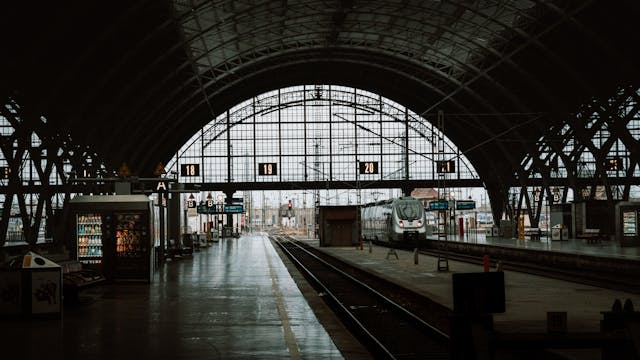
\includegraphics[width = 0.5\textwidth]{image.jpeg}
%     \caption{Cool train station}
%     \label{fig: image}
% \end{figure*}

\end{ZhChapter}